\documentclass[12pt,a5paper]{article}

\usepackage[italian]{babel}
\usepackage[utf8]{inputenc}
\usepackage[T1]{fontenc}
\usepackage[sc]{mathpazo} % Palatino
\usepackage{lmodern} % Latin modern
\renewcommand*\rmdefault{ppl} %Palatino
\linespread{1.05}
\usepackage{graphicx}
\usepackage{tikz}
\usetikzlibrary{calc}
\usetikzlibrary{positioning}
\usepackage{fix-cm}
\usepackage{lipsum}
\usepackage{lettrine}

\parindent=0pt

\usepackage[pages=some]{background}
\backgroundsetup{%
contents={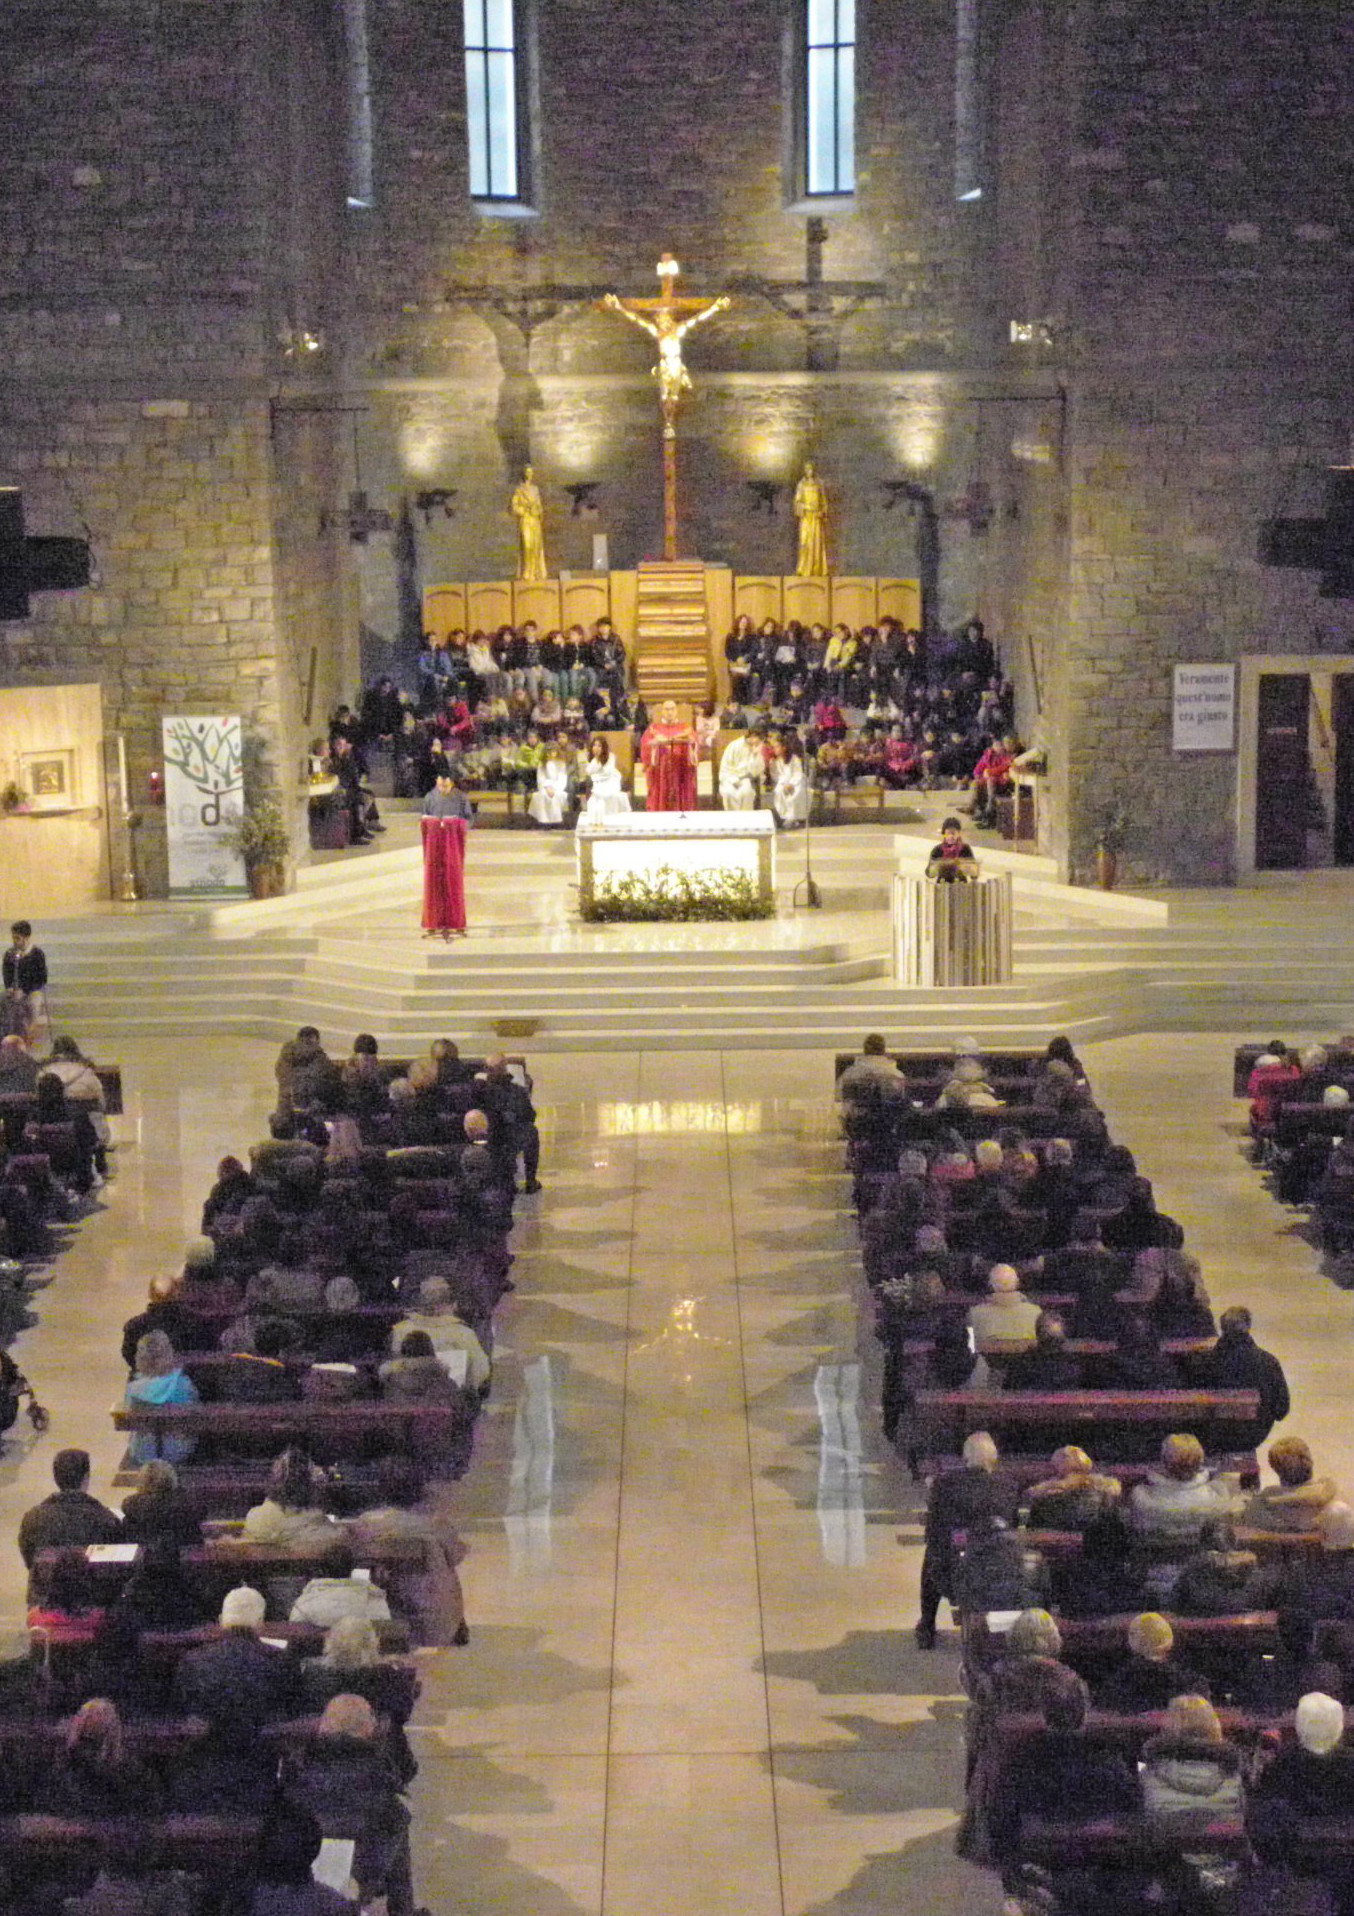
\includegraphics[width=\paperwidth,height=\paperheight]{chiesa}}, 
angle=0,
opacity=1.0,
scale=1
}

\begin{document}
\pagestyle{empty}
\BgThispage
\begin{tikzpicture}[remember picture, overlay]
\node[text width=\paperwidth,anchor=north, minimum width=\paperwidth, minimum height=4.5cm, outer sep=0pt, fill=cyan!50, fill opacity=0.7, text opacity=1, align=center] at (current page.north) {%
\Large{\sffamily PARROCCHIA di SAN FRANCESCO in TRIESTE\par }\bigskip{\fontsize{25}{25}\selectfont\bfseries 1965-2015: 50 ANNI di VITA\par }\bigskip LA COMUNITÀ RACCONTA\par 
};
\node [anchor=south,align=center,fill opacity=0.3] at (current page.south) {
\includegraphics[width=8cm]{tau.png}};
\end{tikzpicture}

\end{document}
